\documentclass[runningheads]{llncs}

%for appendix code
\usepackage{listings}

\lstdefinestyle{pythoncode}{
    language=Python,
    basicstyle=\ttfamily\scriptsize,
    keywordstyle=\bfseries,
    commentstyle=\itshape,
    stringstyle=\ttfamily,
    numbers=left,
    numberstyle=\tiny,
    stepnumber=1,
    numbersep=6pt,
    frame=single,
    breaklines=true,
    breakatwhitespace=false,
    showstringspaces=false,
    tabsize=4,
    captionpos=b
}


\usepackage[T1]{fontenc}
% T1 fonts will be used to generate the final print and online PDFs,
% so please use T1 fonts in your manuscript whenever possible.
% Other font encodings may result in incorrect characters.

\usepackage{placeins}

\usepackage{tabularx}
\newcolumntype{Y}{>{\raggedright\arraybackslash}X}


\usepackage{graphicx}
% Used for including figures.

\usepackage{booktabs}
\usepackage{amsmath,amssymb}

\usepackage{array}
\usepackage{makecell}

\newcolumntype{M}[1]{>{\raggedright\arraybackslash}m{#1}}

\usepackage{array}
\usepackage{makecell}


\newcolumntype{L}[1]{>{\raggedright\arraybackslash}p{#1}}

% Optional URL styling following the LNCS sample comment
\usepackage{xcolor}
\usepackage{hyperref}
\usepackage{array}
\usepackage{makecell}
\usepackage{multirow}
\renewcommand\UrlFont{\color{blue}\rmfamily}

%for tables
\newcolumntype{L}[1]{>{\raggedright\arraybackslash}p{#1}}
\newcolumntype{C}[1]{>{\centering\arraybackslash}p{#1}}
\urlstyle{rm}

\usepackage{longtable}
\usepackage{array}

\newcolumntype{L}[1]{>{\raggedright\arraybackslash}p{#1}}




\raggedbottom

\begin{document}

\title{A Retrieval-Augmented Chatbot for Product Manuals%
}

\titlerunning{Chatbot for Product Manuals}

\author{Duranne Duran \and
Shaina Marie Talisay}

\authorrunning{D. Duran \and S. Talisay}

\institute{University of the Philippines Visayas\\
\email{dbduran@up.edu.ph, sdtalisay@up.edu.ph}}

\maketitle

% \begin{abstract}
% Around 150--250 words.

% \keywords{News credibility \and Supervised learning \and Machine learning \and Model comparison}
% \end{abstract}

\section{Introduction}

\subsection{Background}

Product manuals are intended to guide users in operating, maintaining, and troubleshooting appliances and devices. However, these manuals are often distributed as long PDF documents containing dense technical instructions, diagrams, warnings, and troubleshooting tables. For users who need quick answers to specific problems, manually searching through these documents can be time-consuming and difficult. Traditional keyword search may also fail when users describe their problems in everyday language instead of using the exact terms found in the manual.

Retrieval-Augmented Generation, or RAG, combines document retrieval with a language model. Instead of relying only on the language model's stored knowledge, a RAG system first retrieves relevant passages from a document collection and then generates an answer based on those retrieved passages.

In this project, the system applies RAG to product user manuals. The system processes appliance manuals, converts their text into vector embeddings, stores them in a searchable vector database, retrieves relevant chunks based on the user's question, and generates a grounded response using a language model. It also includes an automatic manual-classification component that predicts which manual a user's question is about, reducing the need for users to manually select the correct source document.

\subsection{Project Statement}

Users often struggle to find specific troubleshooting or procedural information in product manuals because these documents are lengthy, technical, and difficult to search using natural language queries. The wording used by users may differ from the exact terms used in the manual, making relevant information harder to locate.

This project addresses the problem by developing a retrieval-augmented chatbot that retrieves relevant passages from multiple appliance manuals and generates grounded natural-language answers. It also evaluates different RAG pipeline configurations using automatic scoring, human review, and RAGAS metrics to assess retrieval quality, answer relevance, and faithfulness to the source material.

\subsection{Project Objectives}

The general objective of this project is to develop and evaluate a retrieval-augmented chatbot that can answer user questions grounded in product manuals.

Specifically, the project aims to:

\begin{enumerate}
    \item Design and implement a RAG-based question-answering pipeline for multiple appliance manuals.

    \item Generate vector embeddings for manual chunks using transformer-based sentence embedding models.

    \item Store and retrieve relevant manual passages using a vector database.

    \item Train a small feed-forward classifier to predict the correct manual for a given user query.

    \item Compare different RAG pipeline variants in terms of retrieval quality, answer relevance, faithfulness, and latency.

    \item Evaluate the system using multiple methods, including AI-assisted scoring, human review, and RAGAS metrics.

\end{enumerate}

\section{Related Works}

Retrieval-Augmented Generation (RAG) combines document retrieval with language generation, allowing a model to answer using information retrieved from an external corpus rather than relying only on its pretrained knowledge~\cite{lewis2020rag}. This approach is suitable for product manuals because the answer to a user question often exists in the manual, but may be difficult to find through manual browsing or keyword search.

Several related works have applied RAG to technical documentation and manual-based information retrieval. Fredqvist and Sabic~\cite{fredqvist2025ragchatbot} developed a locally hosted RAG chatbot for domain-specific manuals in an ABB Robotics case study. Their system used document preprocessing, embeddings, ChromaDB, retrieval methods such as TF-IDF and BM25, and local Llama models. Their work is closely related to this project because both systems aim to reduce manual searching in technical documents and support local deployment.

Liu et al.~\cite{liu2024automotivepdfchatbots} optimized RAG techniques for automotive industry PDF chatbots using locally deployed Ollama models. Their system addressed PDF processing, retrieval optimization, context compression, reranking, BM25 retrieval, and self-RAG for technical automotive documents. This is similar to the present project because both use local models and compare retrieval configurations for document-grounded question answering. However, the present system focuses on household and office product manuals instead of automotive industry documents.

Yildirim and Samli~\cite{yildirim2025automotiveassistant} developed a RAG-based conversational assistant for the automotive sector. Their assistant supported vehicle owners and service professionals by providing real-time, context-aware information for troubleshooting and maintenance. This relates to the current project because both systems use RAG to support users in finding technical support information, although this project focuses on multiple appliance manuals rather than automotive service data.

Argnani~\cite{argnani2025firmwaremanuals} explored a domain-specific RAG chatbot for firmware manuals. The study emphasized technical correctness, traceability, and the need for users to verify answers against relevant manual sections. This is relevant to the present work because product manual chatbots must not only generate fluent answers, but also remain grounded in source documents and provide references.

Hindy and Denton~\cite{hindy2024instructionmanual} extended RAG to instruction manual understanding using a multimodal approach with contrastive learning. Their work focuses on retrieving visual information from instruction manuals, while the present project is text-based. Nevertheless, it highlights an important direction for future improvement, since many product manuals contain diagrams, tables, and images that are not fully captured by text extraction alone.

Prior studies show that RAG is a practical approach for technical documentation, product support, and manual-based question answering. The present project differs by focusing on five appliance and office-equipment manuals, comparing three local RAG pipeline variants, and adding a trained manual classifier to automatically route user queries to the correct source manual.

\section{Methodology}

The overall workflow of the system is shown in Figure~\ref{fig:system-architecture}.

\begin{figure}[htbp]
    \centering
    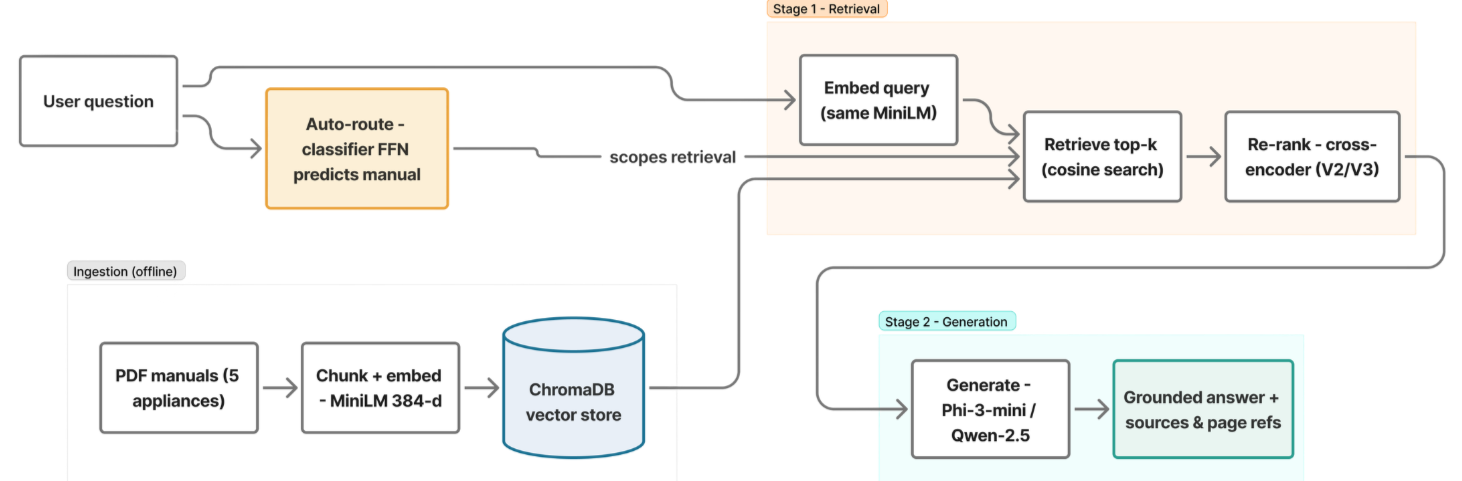
\includegraphics[width=\textwidth]{figures/system_archi.png}
    \caption{System architecture of the retrieval-augmented chatbot for product manuals.}
    \label{fig:system-architecture}
\end{figure}

\subsection{Manual Ingestion and Text Processing}

The product manuals were stored as PDF files inside the \texttt{backend/manuals/} directory. The system used the \texttt{pypdf} library to extract text from each PDF page. During extraction, whitespace and repeated line breaks were normalized to reduce formatting noise from the original manuals.

After text extraction, each page was divided into overlapping text chunks. In the final retrieval setup, the chunk size was set to 500 characters with an overlap of 80 characters. This overlap was used so that important information near chunk boundaries would not be completely separated. Each chunk was stored together with its source filename and page number as metadata.

\subsection{Manual Corpus}

The system used five product manuals as its document corpus as shown in Table~\ref{tab:manual-corpus}. These manuals were placed in the \texttt{backend/manuals/} directory and were indexed for retrieval. 

\begin{table}[htbp]
\centering
\caption{Product manuals included in the RAG corpus}
\label{tab:manual-corpus}
\small
\setlength{\tabcolsep}{4pt}
\renewcommand{\arraystretch}{1.15}

\begin{tabularx}{\textwidth}{@{}p{2.4cm}Y p{4.1cm}@{}}
\toprule
\textbf{Category} & \textbf{Manual} & \textbf{Filename} \\
\midrule

Air conditioner &
Panasonic Air Conditioner Service Manual for CS-NZ25YKE, CS-NZ35YKE, CS-NZ50YKE, CU-NZ25YKE, CU-NZ35YKE, and CU-NZ50YKE &
\texttt{Service-Manual-18.pdf} \\

Printer &
HP LaserJet Pro MFP M329, M428--M429 User Guide &
\texttt{c06184015.pdf} \\

Printer &
Epson ET-4850 User's Guide &
\texttt{cpd60205.pdf} \\

Refrigerator &
Samsung Refrigerator User Manual for RF32CG, RF27CG, and RF70F27 series &
\begin{minipage}[t]{4.1cm}
\ttfamily\footnotesize
DA68-04752Q\_FDR\_RF6500C\_\\3Door\_EN\_MES\_CFR\_260209.pdf
\end{minipage} \\

Washing machine &
LG Washing Machine Owner's Manual for WM4200H*A and WM4000H*A &
\texttt{db05a9.pdf} \\

\bottomrule
\end{tabularx}
\end{table}

\subsection{Embedding and Vector Storage}

Each text chunk was converted into a dense vector representation using the \texttt{sentence-transformers} library. The final embedding model used for retrieval was \texttt{BAAI/bge-small-en-v1.5}, which produces 384-dimensional embeddings. The embeddings were normalized so that cosine similarity could be used during vector search.

The vector embeddings, chunk text, source filename, and page metadata were stored in a persistent \texttt{ChromaDB} collection. The ChromaDB collection was configured to use cosine similarity for comparing query and document embeddings.

\subsection{Retrieval and Re-ranking}

In the final setup, the retriever first obtains up to 20 candidate chunks from ChromaDB.

To improve the quality of the retrieved context, the system applies a second-stage re-ranking process using the \texttt{cross-encoder/ms-marco-MiniLM-L-6-v2} model. Unlike the embedding model, which compares query and document vectors separately, the cross-encoder evaluates each query-chunk pair together and assigns a relevance score. The system then sorts the retrieved candidates by this score and returns the top \texttt{k} chunks, with \texttt{top\_k = 4} used as the default setting.

The retrieval process also supports source filtering. If a specific manual filename is provided, ChromaDB only retrieves chunks from that manual. This prevents the chatbot from mixing information from different appliance manuals.

\subsection{Answer Generation}

The retrieved chunks are passed to a generator model, which produces the final natural-language answer. The generator was implemented in \texttt{generator.py} with two interchangeable backends.

The first backend uses Hugging Face Transformers with PyTorch to run \texttt{microsoft/Phi-3-mini-4k-instruct}. This served as the main generator for the baseline and improved retrieval variants. The second backend uses a local Ollama server through the endpoint \texttt{http://localhost:11434/api/generate}, with \texttt{qwen2.5:3b} as the generator model.

Both generator backends use the same system prompt. The prompt instructs the model to answer only from the retrieved manual context, avoid unsupported claims, avoid telling the user to consult the manual, and avoid adding filenames or page numbers inside the generated answer. The system uses greedy decoding by setting the temperature to 0.0 to make responses more consistent for factual manual-based question answering.

After generation, the response is passed through a post-processing step in \texttt{rag\_pipeline.py}. This step removes any model-generated inline citations such as fabricated filename-page references. Instead of relying on the model to cite sources, the system returns structured source records based on retriever metadata.

\subsection{API and Frontend Implementation}

The backend was implemented using \texttt{FastAPI}. The API was run locally using \texttt{Uvicorn}. The main API endpoints were:

\begin{enumerate}
    \item \texttt{GET /health} -- checks whether the backend is running.
    \item \texttt{GET /sources} -- returns the list of indexed manual filenames.
    \item \texttt{POST /ingest} -- rebuilds the ChromaDB index from the PDF manuals.
    \item \texttt{POST /ask} -- performs retrieval and answer generation.
    \item \texttt{POST /classify} -- predicts which manual a query belongs to.
    \item \texttt{POST /ask\_auto} -- automatically classifies the query, routes it to the predicted manual, and generates an answer.
\end{enumerate}

The frontend was developed using Vite and React. It provides a chat interface where users can type questions, select the generator backend, and view the generated answer with its retrieved sources. The frontend first calls the classifier endpoint to route the query, then sends the question to the \texttt{/ask} endpoint using the predicted manual as the source filter.

\subsection{Manual Classification}

To reduce the need for users to manually select a product manual, the system includes a manual classifier implemented in \texttt{manual\_classifier.py}. The classifier uses frozen \texttt{sentence-transformers/all-MiniLM-L6-v2} embeddings as input. The embedding output is a 384-dimensional vector.

A small feed-forward neural network was trained on top of these frozen embeddings. The classifier architecture was:

\[
\text{Linear}(384 \rightarrow 128) \rightarrow \text{ReLU} \rightarrow \text{Dropout}(0.2) \rightarrow \text{Linear}(128 \rightarrow 5)
\]

The five output classes correspond to the five appliance manuals. The output logits are passed through a softmax function to obtain the probability of each manual. The predicted manual is the class with the highest probability.

The classifier was trained using cross-entropy loss and the Adam optimizer. The training data came from the manually prepared evaluation questions and was expanded through deterministic paraphrasing and synonym substitution, such as replacing ``washer'' with ``washing machine'' or ``air conditioner'' with ``AC''. This allowed the classifier to learn common variations in user wording.

\subsection{Pipeline Variants}

Three pipeline variants were implemented and compared:

\begin{enumerate}
    \item \textbf{V1 Baseline} -- used \texttt{sentence-transformers/all-MiniLM-L6-v2}, 800-character chunks with 120-character overlap, no re-ranker, and \texttt{Phi-3-mini} as the generator.
    
    \item \textbf{V2 Improved Retrieval} -- used \texttt{BAAI/bge-small-en-v1.5}, 500-character chunks with 80-character overlap, \texttt{cross-encoder/ms-marco-MiniLM-L-6-v2} as the re-ranker, and \texttt{Phi-3-mini} as the generator.
    
    \item \textbf{V3 Alternative Generator} -- used the same retrieval setup as V2 but replaced \texttt{Phi-3-mini} with \texttt{qwen2.5:3b} through Ollama.
\end{enumerate}

This experimental setup allowed the project to compare whether improvements in retrieval or changes in the generator had a greater effect on answer quality.

\subsection{Evaluation Procedure}

The system was evaluated using a 25-question evaluation set. The questions covered five product manuals and included procedural, factual, and tricky troubleshooting questions. Each question had a manually written reference answer.

The script \texttt{run\_eval.py} was used to send each question to the running FastAPI backend through the \texttt{/ask} endpoint. For each question, the script recorded the generated answer, retrieved sources, response latency, status code, and any error message into a CSV file.

The generated answers were evaluated using three methods. First, \texttt{qwen2.5:3b} was used through Ollama as a local AI judge. The judge classified each answer as \textit{Correct}, \textit{Partial}, \textit{Wrong}, or \textit{Refused}. Second, human review was conducted by manually comparing generated answers with the reference answers and source manuals. Third, \texttt{run\_ragas.py} used RAGAS to compute four metrics: faithfulness, answer relevancy, context precision, and context recall.

For RAGAS evaluation, the judge model was \texttt{qwen2.5:3b} through Ollama, while \texttt{sentence-transformers/all-MiniLM-L6-v2} was used for response relevancy embeddings. The evaluation outputs were saved as per-question CSV files and summary JSON files for each pipeline variant.


\section{Results and Discussion}

\subsection{Comparison of RAG Pipeline Variants}

The three pipeline variants were evaluated using RAGAS metrics. V1 served as the baseline configuration, V2 tested the effect of retrieval improvements, and V3 tested the effect of changing the generator while keeping the V2 retrieval setup. The results are shown in Table~\ref{tab:ragas-comparison} and Figure~\ref{fig:ragas-metrics}.

\begin{table}[htbp]
\centering
\caption{RAGAS comparison of the three pipeline variants}
\label{tab:ragas-comparison}
\small
\setlength{\tabcolsep}{3pt}
\renewcommand{\arraystretch}{1.15}
\begin{tabularx}{\textwidth}{@{}p{3.1cm}C{1.9cm}C{1.9cm}C{1.9cm}C{1.9cm}C{1.7cm}@{}}
\toprule
\textbf{Variant} & \textbf{Faithfulness} & \textbf{Answer Relevancy} & \textbf{Context Precision} & \textbf{Context Recall} \\
\midrule
V1 Baseline & 0.184 (n=14) & 0.721 & 0.861 & 0.904 (n=22) \\
V2 Improved Retrieval & 0.448 (n=19) & 0.732 & 0.856 & 0.663 (n=19) \\
V3 Alternative Generator & 0.378 (n$\approx$17) & 0.513 & 0.852 & 0.663 (n$\approx$19) \\
\bottomrule
\end{tabularx}
\end{table}

The results show that retrieval was generally effective across all variants. Context precision remained high, with all variants scoring above 0.85. This means that the retrieved chunks were usually relevant to the user questions. However, faithfulness was much lower than context precision, especially in the baseline. V1 achieved a context precision of 0.861 and context recall of 0.904, but its faithfulness score was only 0.184. This indicates that the system often retrieved useful manual content, but the generator did not always produce answers that were fully supported by the retrieved passages.

The comparison between V1 and V2 shows the effect of improving the retrieval stage. V2 increased faithfulness from 0.184 to 0.448, which suggests that the use of BGE embeddings, smaller chunks, and a cross-encoder re-ranker helped the generator produce more grounded answers. However, context recall decreased from 0.904 to 0.663. This suggests that smaller chunks made the retrieved context more focused but less likely to contain complete multi-step procedures from the manuals.

The comparison between V2 and V3 shows the effect of changing the generator. V3 used the same retrieval setup as V2 but replaced Phi-3-mini with Qwen-2.5-3B through Ollama. Since context precision and context recall remained almost unchanged, the decrease in faithfulness and answer relevancy can be attributed mainly to the generator. V3 had lower answer relevancy, decreasing from 0.732 to 0.513, showing that Qwen-2.5-3B produced less focused answers for this task.

A runtime difference was also observed between the two generator backends. When generation was run on an NVIDIA RTX 3050 GPU, the Ollama-based Qwen-2.5-3B backend generated an answer in approximately 48 seconds, while the Hugging Face Transformers backend using Phi-3-mini took about 3 minutes. This shows that although Qwen-2.5-3B had lower answer relevancy in the evaluation, it produced responses faster in the tested local GPU environment. Therefore, the generator choice involved a trade-off between answer quality and generation speed.


\begin{figure}[htbp]
    \centering
    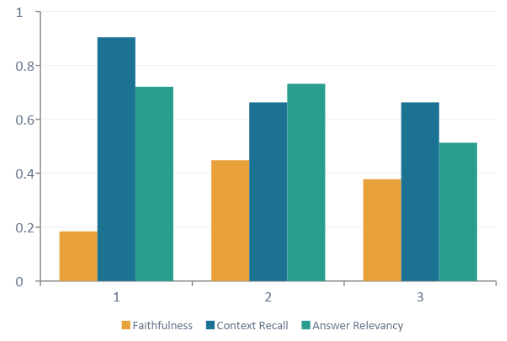
\includegraphics[width=0.85\textwidth]{figures/ragas_metrics.png}
    \caption{RAGAS metric comparison across the three pipeline variants.}
    \label{fig:ragas-metrics}
\end{figure}

\subsection{AI-Assisted Scoring and Human Review}

Aside from RAGAS, the V1 baseline was also evaluated using AI-assisted scoring and human review. The AI-assisted scoring used Qwen-2.5-3B as a local judge, while human review involved manually comparing the generated answers with the reference answers and source manuals. The results are shown in Table~\ref{tab:qwen-human}.

\begin{table}[t]
\centering
\caption{Comparison of AI-assisted scoring and human review for V1}
\label{tab:qwen-human}
\small
\setlength{\tabcolsep}{5pt}
\renewcommand{\arraystretch}{1.15}
\begin{tabularx}{0.85\textwidth}{@{}Y C{2.5cm} C{2.5cm}@{}}
\toprule
\textbf{Scoring Method} & \textbf{Strict Accuracy} & \textbf{Lenient Accuracy} \\
\midrule
Qwen-2.5-3B judge & 4\% & 26\% \\
Human review & 28\% & 50\% \\
\bottomrule
\end{tabularx}
\end{table}

The AI-assisted judge scored the baseline much lower than the human reviewers. Qwen-2.5-3B gave a strict accuracy of 4\%, while human review gave 28\%. For lenient accuracy, which gives partial credit to incomplete but relevant answers, Qwen gave 26\%, while human review gave 50\%.

This difference shows that the local LLM judge was stricter than human evaluation. The judge tended to penalize answers that missed exact details, even when the answer still contained relevant and useful information. Because of this, AI-assisted scoring was treated as a supporting evaluation method rather than the only basis for assessing system quality. Human review remained necessary to determine whether the answers were practically useful and aligned with the source manuals.

\subsection{Manual Classifier Results}

The manual classifier was evaluated using 5-fold cross-validation. It was trained to predict which manual a user query belongs to, allowing the system to automatically route questions before retrieval. The results are shown in Table~\ref{tab:classifier-results}.

\begin{table}[t]
\centering
\caption{Manual classifier validation accuracy}
\label{tab:classifier-results}
\small
\setlength{\tabcolsep}{6pt}
\renewcommand{\arraystretch}{1.15}
\begin{tabular}{@{}C{3cm} C{4cm}@{}}
\toprule
\textbf{Fold} & \textbf{Validation Accuracy} \\
\midrule
1 & 1.000 \\
2 & 1.000 \\
3 & 1.000 \\
4 & 0.950 \\
5 & 0.950 \\
\midrule
Mean & 0.980 $\pm$ 0.024 \\
\bottomrule
\end{tabular}
\end{table}

The classifier achieved a mean validation accuracy of 0.980 with a standard deviation of 0.024. This shows that the classifier was effective at identifying the correct manual within the prepared dataset. Its integration into the \texttt{/ask\_auto} endpoint improves usability because users do not need to manually select the correct product manual before asking a question.

However, this result should be interpreted with caution. The training data was expanded through deterministic paraphrasing, and cross-validation was performed over the augmented examples. This means that paraphrases of the same original question may appear in both training and validation folds. As a result, the reported accuracy is likely an upper-bound estimate. A stricter evaluation should group paraphrases of the same original question into the same fold.


\section{Conclusion}

The results show that the system can retrieve relevant information from multiple product manuals, but answer generation remains the main challenge. Although the retriever achieved high context precision, the lower faithfulness scores indicate that the generator sometimes produced unsupported, incomplete, or less focused answers.

Among the three variants, V2 produced the best grounding performance. V2 refers to the improved retrieval configuration that used \texttt{BAAI/bge-small-en-v1.5} for embeddings, 500-character chunks with 80-character overlap, \texttt{cross-encoder/\newline ms-marco-MiniLM-L-6-v2} for re-ranking, and \texttt{Phi-3-mini} as the generator. This setup increased faithfulness, showing that better context selection can reduce unsupported generation. However, its lower context recall suggests that smaller chunks may lose useful surrounding information, especially for longer step-by-step procedures.

The generator comparison also showed that model choice affects both answer quality and runtime. Qwen-2.5-3B did not outperform Phi-3-mini in answer quality, suggesting that stronger models, fine-tuning, or more controlled prompting may be needed to improve generated answers. However, Qwen-2.5-3B through Ollama was faster in the tested local environment, generating responses in approximately 48 seconds while Phi-3-mini through Hugging Face Transformers took about 3 minutes. 

The evaluation also showed that scoring method affects the reported results. The Qwen-based judge gave lower scores than human review, indicating that small local LLMs may be too strict or inconsistent as standalone evaluators. Using multiple evaluation methods therefore provided a more balanced assessment of the system.

Overall, the project demonstrates that a RAG-based chatbot can make product manuals easier to use by retrieving relevant passages and generating direct answers. The strongest component of the system is retrieval, while the main area for improvement is generating answers that are fully faithful, complete, and focused on the retrieved manual context.

For future work, the system may be improved through hybrid chunking, where shorter chunks are used for specific troubleshooting facts and larger merged chunks are used for complete procedures. Future versions may also test stronger or fine-tuned generator models, evaluate the manual classifier using stricter data splits, support scanned manuals through OCR, add streaming responses and conversational memory, and use a larger evaluation set for more reliable performance measurement.


% \input{sections/06-appendix}

% \begin{credits}
% \subsubsection{\ackname}
% Add funding, institutional, or project acknowledgements here.

% \subsubsection{\discintname}
% The authors have no competing interests to declare that are relevant to the content of this article.
% \end{credits}

\input{sections/appendix}

\bibliographystyle{splncs04}
\bibliography{refs}


\end{document}